\documentclass[11.95pt,a4paper]{article}

\usepackage{amsmath,amssymb,amsthm}
\usepackage{}
\usepackage{multicol}
\usepackage[framemethod=TikZ]{mdframed}
\usepackage[T5]{fontenc}
\usepackage[utf8]{inputenc}
\usepackage[vietnamese,english]{babel}
\usepackage{amsmath}
\usepackage{graphicx}
\usepackage[colorinlistoftodos]{todonotes}
\usepackage{listings}
\usepackage{hyperref}
\usepackage{float}
\usepackage{enumitem}
\usepackage{minted}
\usepackage{forest}
\hypersetup{
    colorlinks=true,
    linkcolor=blue,
    filecolor=magenta,
    urlcolor=cyan,
}
\usepackage{tikz} 
\usepackage{scrextend}
\usepackage{fancyhdr}
\usepackage{mathrsfs}
\usepackage{amssymb}

\usepackage[utf8]{inputenc}
\usepackage[T1]{fontenc}
\usepackage[margin=2.3cm]{geometry}
\usepackage{lmodern}
\usepackage{microtype}
\usepackage{graphicx}
\usepackage{booktabs}
\usepackage{longtable}
\usepackage{array}
\usepackage{tabularx}
\usepackage{enumitem}
\usepackage{xcolor}
\usepackage{listings}
\usepackage{amsmath,amssymb}
\usepackage{float}
\usepackage{fancyhdr}
\usepackage{hyperref}
\usepackage{tikz}
\usetikzlibrary{arrows.meta,positioning,shapes.geometric,fit}

\definecolor{linkblue}{RGB}{0,35,180}
\definecolor{codebg}{RGB}{247,248,250}
\hypersetup{
  colorlinks=true,
  linkcolor=linkblue,
  urlcolor=linkblue,
  citecolor=linkblue,
  pdftitle={Hybrid FTP Application Technical Report}
}

\pagestyle{fancy}
\fancyhf{}
\lhead{Internetworking Protocol}
\rhead{Hybrid FTP Application}
\cfoot{\thepage}
\setlength{\headheight}{15pt}
\setlength{\parindent}{0pt}
\setlength{\parskip}{0.55em}
\setlist{nosep}
\renewcommand{\arraystretch}{1.2}

\lstset{
  basicstyle=\ttfamily\small,
  backgroundcolor=\color{codebg},
  frame=single,
  breaklines=true,
  columns=fullflexible,
  keepspaces=true,
  showstringspaces=false
}

\def\ojoin{\setbox0=\hbox{$\bowtie$}%
  \rule[-.02ex]{.25em}{.4pt}\llap{\rule[\ht0]{.25em}{.4pt}}}
\def\leftouterjoin{\mathbin{\ojoin\mkern-5.8mu\bowtie}}
\def\rightouterjoin{\mathbin{\bowtie\mkern-5.8mu\ojoin}}
\def\fullouterjoin{\mathbin{\ojoin\mkern-5.8mu\bowtie\mkern-5.8mu\ojoin}}

\usepackage{xcolor}

\definecolor{codegreen}{rgb}{0,0.6,0}
\definecolor{codegray}{rgb}{0.5,0.5,0.5}
\definecolor{codepurple}{rgb}{0.58,0,0.82}
\definecolor{backcolour}{rgb}{0.95,0.95,0.92}

\lstdefinestyle{mystyle}{
    backgroundcolor=\color{backcolour},   
    commentstyle=\color{codegreen},
    keywordstyle=\color{magenta},
    numberstyle=\tiny\color{codegray},
    stringstyle=\color{codepurple},
    basicstyle=\ttfamily\normalsize,
    breakatwhitespace=false,         
    breaklines=true,                 
    captionpos=b,                    
    keepspaces=true,                 
    numbers=left,                    
    numbersep=5pt,
    showspaces=false,                
    showstringspaces=false,
    showtabs=false,                  
    tabsize=2
}
\lstset{style=mystyle}

\newcommand{\placeholder}[1]{\textcolor{red}{[#1]}}
\newcommand{\code}[1]{\texttt{\detokenize{#1}}}
\newcommand{\pass}{\textbf{\textcolor{green!50!black}{PASS}}}

\pagestyle{fancy}
\fancyhf{}
\rhead[top=30mm]{Project 1 -- CS333}
\lhead[top=30mm]{22125118 -- 23125055}
\rfoot{Page \thepage}

\title{test}
\author{Nguyen Hoang Gia Han}
\date{October 2023}

\begin{document}

\begin{titlepage}
%\SetWatermarkText{\includegraphics[width = 0.97\paperwidth,
%height = 0.97\paperheight]{bia.png}}
%\SetWatermarkAngle{0} 
%\SetWatermarkText{\includegraphics[scale=1]{hust.png}}
%\SetWatermarkAngle{0} 
\begin{tikzpicture}[remember picture,overlay,inner sep=0,outer sep=0]
     \draw[blue!70!black,line width=4pt] ([xshift=-1.5cm,yshift=-2cm]current page.north east) coordinate (A)--([xshift=1.5cm,yshift=-2cm]current page.north west) coordinate(B)--([xshift=1.5cm,yshift=2cm]current page.south west) coordinate (C)--([xshift=-1.5cm,yshift=2cm]current page.south east) coordinate(D)--cycle;

     \draw ([yshift=0.5cm,xshift=-0.5cm]A)-- ([yshift=0.5cm,xshift=0.5cm]B)--
     ([yshift=-0.5cm,xshift=0.5cm]B) --([yshift=-0.5cm,xshift=-0.5cm]B)--([yshift=0.5cm,xshift=-0.5cm]C)--([yshift=0.5cm,xshift=0.5cm]C)--([yshift=-0.5cm,xshift=0.5cm]C)-- ([yshift=-0.5cm,xshift=-0.5cm]D)--([yshift=0.5cm,xshift=-0.5cm]D)--([yshift=0.5cm,xshift=0.5cm]D)--([yshift=-0.5cm,xshift=0.5cm]A)--([yshift=-0.5cm,xshift=-0.5cm]A)--([yshift=0.5cm,xshift=-0.5cm]A);


     \draw ([yshift=-0.3cm,xshift=0.3cm]A)-- ([yshift=-0.3cm,xshift=-0.3cm]B)--
     ([yshift=0.3cm,xshift=-0.3cm]B) --([yshift=0.3cm,xshift=0.3cm]B)--([yshift=-0.3cm,xshift=0.3cm]C)--([yshift=-0.3cm,xshift=-0.3cm]C)--([yshift=0.3cm,xshift=-0.3cm]C)-- ([yshift=0.3cm,xshift=0.3cm]D)--([yshift=-0.3cm,xshift=0.3cm]D)--([yshift=-0.3cm,xshift=-0.3cm]D)--([yshift=0.3cm,xshift=-0.3cm]A)--([yshift=0.3cm,xshift=0.3cm]A)--([yshift=-0.3cm,xshift=0.3cm]A);

   \end{tikzpicture}
\begin{center}
    \vspace{1pt}
    \fontsize{13pt}{17pt}\selectfont 
    \textbf{VNUHCM – UNIVERSITY OF SCIENCE}
    
    \vspace{7pt}
    \textbf{ADVANCED PROGRAM IN COMPUTER SCIENCE}
\end{center}
\vspace{1cm}
\begin{center}
    
\includegraphics[scale=0.55]{logo-khtn.png}
    
    \vspace{10pt}
    \fontsize{30pt}{17pt}\selectfont 
    
    \vspace{50pt}
    \textbf{Project 1: Socket Programming}

\begin{flushleft}
    \fontsize{14pt}{17pt}\selectfont  
\end{flushleft}

    \fontsize{15pt}{17pt}\selectfont 
    \textbf{\textrm{Internetworking Protocols}}


\vspace*{7cm} 
{\large\bf 23125055 -- Nguyen Hoang Gia Han}\\

\vspace*{0.5cm} 
{\large\bf 23125043 -- Nguyen Van Hoang Nhat}\\

\end{center}
\end{titlepage}
\fontsize{13pt}{17pt}\selectfont
\tableofcontents
\newpage
\section*{Self-Assessment}
\setlength{\tabcolsep}{12pt} % Adjusts horizontal padding
\renewcommand{\arraystretch}{1.6} % Adjusts vertical padding

\begin{table}[H]
\centering
\begin{tabular}{|c|l|c|}
\hline
\textbf{No} & \textbf{Name} & \textbf{Contribution} \\ \hline
1           &  Nguyen Hoang Gia Han          & 50\%                     \\ \hline
2           & Nguyen Van Hoang Nhat          & 50\%                  \\ \hline
\end{tabular}
\caption{Self-assessment table}
\end{table}


\section{Application Scenario \& Protocol Interaction}
\subsection{Application scenario}
The application is a command-line Hybrid FTP system that separates the
control and data planes. FTP commands, standard three-digit replies,
authentication, and session state use a persistent TCP connection. File
contents and directory listings use UDP with a custom application-layer
Go-Back-N reliability protocol.

The server listens at \code{127.0.0.1:2121}. Each accepted TCP connection
creates one independent \code{Session} in one daemon thread. The session owns
the authenticated user, working directory, transfer type, transfer mode,
active/passive endpoint state, rename state, and cancellation event. Server
files are confined to \code{server_files/}; client downloads are written to
\code{client_downloads/}.

\subsection{Architecture}

\begin{figure}[H]
\centering
\begin{tikzpicture}[
  node distance=8mm and 14mm,
  box/.style={draw,rounded corners,align=center,minimum width=45mm,minimum height=9mm},
  arrow/.style={-{Latex[length=2.5mm]},thick}
]
\node[box] (user) {User commands\\login, put, get, ls, verify};
\node[box,below=of user] (cli) {\code{client/client.py}\\Interactive CLI};
\node[box,below=of cli] (fc) {\code{client/ftp_client.py}\\Client protocol API};
\node[box,right=45mm of fc] (server) {\code{server/server.py}\\TCP accept + thread/session};
\node[box,below=of server] (session) {\code{server/session.py}\\Authentication and dispatch};
\node[box,below=18mm of fc,xshift=30mm] (rdt) {\code{common/rdt.py}\\Go-Back-N reliable UDP};
\draw[arrow] (user)--(cli);
\draw[arrow] (cli)--(fc);
\draw[arrow,<->] (fc)--node[above]{TCP commands/replies}(server);
\draw[arrow] (server)--(session);
\draw[arrow,<->] (fc)--node[left]{UDP data/ACK}(rdt);
\draw[arrow,<->] (rdt)--(session);
\end{tikzpicture}
\caption{Project-wide control and data paths.}
\end{figure}

\subsection{Full TCP + UDP lifecycle}

\begin{longtable}{p{0.07\textwidth}p{0.18\textwidth}p{0.18\textwidth}p{0.47\textwidth}}
\toprule
\# & Sender & Receiver & Interaction\\
\midrule
1 & Client & Server & TCP \code{connect()} to port 2121; server replies \code{220}.\\
2 & Client & Server & \code{USER admin}; server replies \code{331}.\\
3 & Client & Server & \code{PASS ********}; server verifies the selected user and replies \code{230}.\\
4 & Client & Server & \code{PASV}; server binds UDP port 50000--51000 and replies \code{227}.\\
5 & Client & Server & \code{STOR remote.bin} over TCP and an UDP \code{RDY} datagram to the PASV endpoint.\\
6 & Server & Client & \code{150 Opening data connection}.\\
7 & Client & Server & Window of UDP DATA packets containing sequence, length, flags, CRC-32 and payload.\\
8 & Server & Client & Cumulative ACK for the highest contiguous sequence. Loss causes timeout/NAK and GBN retransmission.\\
9 & Server & File system & Reassemble, validate representation, and write under \code{server_files/}.\\
10 & Server & Client & \code{226 Transfer complete}.\\
11 & Client & Server & \code{HASH SHA256 remote.bin}; server replies with \code{213} and digest.\\
12 & Client & Client & Calculate local digest and compare end to end.\\
13 & Client & Server & \code{QUIT}; server replies \code{221}, closes sockets, and deregisters the session.\\
\bottomrule
\end{longtable}

\subsection{Passive and active modes}

\textbf{PASV.} The server binds a random UDP socket, sends its endpoint in
\code{227}, and learns the client's UDP endpoint from the client's RDY
datagram. PASV is the default.

\textbf{PORT.} The client binds a UDP socket and advertises it with
\code{PORT h1,h2,h3,h4,p1,p2}. The server stores that endpoint and sends RDY
from its per-transfer UDP socket. The client learns the server endpoint from
that datagram.

\subsection{Approved command coverage}

\begin{tabularx}{\textwidth}{>{\bfseries}p{0.28\textwidth}X}
\toprule
Category & Commands\\
\midrule
Authentication/session & USER, PASS, QUIT, NOOP, HELP\\
Navigation/directories & PWD, CWD, CDUP, MKD, RMD\\
Listing/metadata & LIST, NLST, STAT, SIZE, MDTM\\
Representation/data setup & TYPE, MODE, PORT, PASV\\
File transfer & RETR, STOR, STOU, APPE, ABOR\\
Management/integrity & DELE, RNFR, RNTO, HASH\\
\bottomrule
\end{tabularx}

All 28 commands required by the specification have server dispatch handlers.

\subsection{Evaluation-level mapping}

\begin{longtable}{p{0.15\textwidth}p{0.32\textwidth}p{0.43\textwidth}}
\toprule
Level & Requirement & Implementation\\
\midrule
Basic & Authentication & Stateful USER/PASS on the TCP session\\
Basic & ASCII and upload/download & TYPE A, STOR and RETR\\
Basic & Fixed data mechanism & PASV default\\
Advanced & Binary files & TYPE I, byte-preserving payload\\
Advanced & Directory tree & Navigation, listing, create/remove, metadata\\
Advanced & Active/passive & Runtime PORT/PASV switching\\
Advanced & Concurrency & One thread and Session per TCP client\\
Excellent & Reliable UDP & Sequence, ACK/NAK, CRC, timeout, retransmission\\
Excellent & Flow/congestion control & GBN window, Slow Start, AIMD\\
Excellent & End-to-end integrity & MD5/SHA-256 local/remote comparison\\
\bottomrule
\end{longtable}

\section{Project-Wide Data Structures}
\subsection{TCP control format}

Client commands use \code{COMMAND [argument]\textbackslash r\textbackslash n};
server responses use \code{ddd message\textbackslash r\textbackslash n}.
TCP receive buffers extract complete CRLF-delimited records because TCP is a
byte stream and does not preserve application message boundaries.

\subsection{Custom UDP header}

The binary format string is \code{!IIBBHIH}, network byte order, with an
18-byte header.

\begin{table}[H]
\centering
\begin{tabular}{rllp{0.43\textwidth}}
\toprule
Offset & Field & Size & Meaning\\
\midrule
0 & Sequence number & 4 B & Zero-based DATA packet position\\
4 & ACK number & 4 B & Highest contiguous sequence received\\
8 & Flags & 1 B & SYN/FIN/ACK/NAK/DAT/RDY bitmask\\
9 & Reserved & 1 B & Currently zero\\
10 & Payload length & 2 B & Valid payload bytes, maximum 1452\\
12 & CRC-32 & 4 B & Payload corruption check\\
16 & Transfer ID & 2 B & Discriminator; current flow uses zero\\
18 & Payload & 0--1452 B & File or listing content\\
\bottomrule
\end{tabular}
\caption{Custom reliable UDP packet fields.}
\end{table}

\begin{lstlisting}
0                   1                   2                   3
0 1 2 3 4 5 6 7 8 9 0 1 2 3 4 5 6 7 8 9 0 1 2 3 4 5 6 7 8 9 0 1
+---------------------------------------------------------------+
|                    Sequence Number (32)                       |
+---------------------------------------------------------------+
|                  Acknowledgement Number (32)                  |
+---------------+---------------+-------------------------------+
|   Flags (8)   | Reserved (8)  |      Payload Length (16)      |
+---------------------------------------------------------------+
|                       CRC-32 (32)                             |
+-------------------------------+-------------------------------+
|       Transfer ID (16)        | Payload (0-1452 bytes) ...    |
+-------------------------------+-------------------------------+
\end{lstlisting}

Flag values are SYN \(0x01\), FIN \(0x02\), ACK \(0x04\), NAK \(0x08\),
DAT \(0x10\), and RDY \(0x20\). Maximum packet size is 1470 bytes.

\subsection{Sender, receiver, and timeout state}

\begin{tabularx}{\textwidth}{l l X}
\toprule
State & Initial value & Purpose\\
\midrule
\code{base} & 0 & Oldest unacknowledged sequence\\
\code{next_seq} & 0 & Next unsent sequence\\
\code{cwnd} & 1 packet & Congestion window\\
\code{ssthresh} & window/2 & Slow Start threshold\\
\code{max_window} & 16 & Protocol window ceiling\\
\code{srtt}, \code{rttvar} & unset & Adaptive RTT estimators\\
\code{rto} & 2.0 s & Retransmission timeout, bounded 0.05--10 s\\
\code{expected_seq} & 0 & Receiver's next acceptable sequence\\
\code{pieces} & empty & Ordered receiver fragments\\
\bottomrule
\end{tabularx}

\[
\mathrm{SRTT}\leftarrow(1-\tfrac18)\mathrm{SRTT}+\tfrac18R,
\quad
\mathrm{RTTVAR}\leftarrow(1-\tfrac14)\mathrm{RTTVAR}
 +\tfrac14|\mathrm{SRTT}-R|
\]
\[
\mathrm{RTO}=\operatorname{clamp}
(\mathrm{SRTT}+\max(G,4\mathrm{RTTVAR}),0.05,10)
\]

Retransmitted packets do not contribute RTT samples (Karn's rule).

\subsection{Session management}

The server owns a locked dictionary mapping integer session IDs to
\code{Session} objects. Each session owns its TCP socket, client address,
authentication state, virtual CWD, TYPE, MODE, PASV/PORT state, data socket,
rename source, transfer thread, cancellation event, and TCP receive buffer.

\subsection{Representation and safety}

\code{TYPE I} preserves bytes. \code{TYPE A} canonicalises network CRLF.
\code{MODE C} applies zlib compression around reliable UDP. Paths are
normalised and checked with \code{os.path.commonpath()} before file access.
HASH supports MD5 and SHA-256.
\section{Functional Workflows (Flowcharts)}

\subsection{Server dispatch}

\begin{figure}[H]
\centering
\begin{tikzpicture}[
  node distance=6mm,
  every node/.style={font=\small},
  proc/.style={draw,rounded corners,align=center,minimum width=47mm,minimum height=7mm},
  decision/.style={draw,diamond,aspect=2,align=center},
  arr/.style={-{Latex},thick}
]
\node[proc] (start) {Bind TCP socket and listen};
\node[proc,below=of start] (accept) {accept client; allocate session ID};
\node[proc,below=of accept] (thread) {Register Session; start daemon thread};
\node[proc,below=of thread] (recv) {Send 220; receive buffered command};
\node[decision,below=of recv] (auth) {Allowed in current\\authentication state?};
\node[proc,below left=8mm and 12mm of auth] (deny) {Reply 530/503};
\node[proc,below right=8mm and 12mm of auth] (dispatch) {Dispatch command handler};
\node[decision,below=16mm of auth] (end) {QUIT, error,\\or disconnect?};
\node[proc,below=of end] (clean) {Cancel transfer; close sockets; deregister};
\draw[arr] (start)--(accept);
\draw[arr] (accept)--(thread);
\draw[arr] (thread)--(recv);
\draw[arr] (recv)--(auth);
\draw[arr] (auth)--node[above left]{no}(deny);
\draw[arr] (auth)--node[above right]{yes}(dispatch);
\draw[arr] (deny)--(end);
\draw[arr] (dispatch)--(end);
\draw[arr] (end.east) -- ++(12mm,0) |- node[pos=.25,right]{no} (recv.east);
\draw[arr] (end)--node[right]{yes}(clean);
\end{tikzpicture}
\caption{TCP accept, authentication gate, and command dispatch.}
\end{figure}

\subsection{Go-Back-N sender}

\begin{figure}[H]
\centering
\begin{tikzpicture}[
 node distance=6mm,
 every node/.style={font=\small},
 proc/.style={draw,rounded corners,align=center,minimum width=55mm,minimum height=7mm},
 decision/.style={draw,diamond,aspect=2,align=center},
 arr/.style={-{Latex},thick}
]
\node[proc] (prep) {Fragment payload; build DATA packets; FIN on last};
\node[proc,below=of prep] (send) {Fill window: base to base + floor(cwnd)};
\node[decision,below=of send] (event) {ACK, NAK, or RTO?};
\node[proc,below left=9mm and 18mm of event] (ack) {ACK: advance base; update RTO if unambiguous};
\node[proc,below right=9mm and 18mm of event] (loss) {Loss: halve threshold/window; timeout resets cwnd to 1};
\node[proc,below=22mm of event] (update) {ACK: Slow Start or additive increase\\Loss: retransmit outstanding flight};
\node[decision,below=of update] (done) {All packets ACKed?};
\node[proc,below=of done] (ok) {Return success};
\draw[arr] (prep)--(send);
\draw[arr] (send)--(event);
\draw[arr] (event)--node[above left]{ACK}(ack);
\draw[arr] (event)--node[above right]{NAK/RTO}(loss);
\draw[arr] (ack)--(update);
\draw[arr] (loss)--(update);
\draw[arr] (update)--(done);
\draw[arr] (done.east)--++(13mm,0)|-node[pos=.2,right]{no}(send.east);
\draw[arr] (done)--node[right]{yes}(ok);
\end{tikzpicture}
\caption{Cumulative-ACK Go-Back-N sender with congestion response.}
\end{figure}

\subsection{Go-Back-N receiver}

The receiver validates header length and CRC, filters the transfer ID and DAT
flag, accepts only \code{seq == expected_seq}, appends that payload, and
returns a cumulative ACK. Corruption produces NAK. Duplicate/future packets
are discarded and the highest contiguous ACK is repeated. FIN on an accepted
packet terminates reassembly.

\subsection{Data-mode toggle and transfer}

PASV binds at the server and uses client-to-server RDY; PORT binds at the
client and uses server-to-client RDY. Both converge on the same
\code{RDTSender}/\code{RDTReceiver} workflow, then release the per-transfer
UDP socket and return \code{226} or \code{426}.

\subsection{Limitations}

Authentication is basic and has no TLS/password hashing. CRC-32 detects
accidental corruption but is not an HMAC. MODE B is accepted but does not
introduce separate RFC block framing. Hash verification is available but not
forced after every transfer. Payloads are assembled in memory. There is no
per-filename write lock. The Slow Start/AIMD design is educational rather
than a complete TCP congestion-control implementation.
\section{Task Assignment Matrix}

\begin{longtable}{p{0.32\textwidth}p{0.15\textwidth}p{0.15\textwidth}p{0.20\textwidth}}
\toprule
Component & Owner & Collaborator & File\\
\midrule
Requirements and architecture & Both & Both & README, report\\
Packet header and constants & Gia Han & Hoang Nhat & common/protocol.py\\
GBN sender and receiver & Gia Han & Hoang Nhat & common/rdt.py\\
Slow Start, AIMD, adaptive RTO & Gia Han & Hoang Nhat & common/rdt.py\\
Hash, ASCII, listing utilities & Hoang Nhat & Gia Han & common/utils.py\\
Authentication and dispatcher & Gia Han & Hoang Nhat & server/session.py\\
PASV/PORT and server data path & Gia Han & Hoang Nhat & server/session.py\\
Threaded server/session table & Gia Han & Hoang Nhat & server/server.py\\
File and directory operations & Hoang Nhat & Gia Han & server/session.py\\
Client protocol API and CLI & Hoang Nhat & Gia Han & client modules\\
Unit tests & Hoang Nhat & Gia Han & tests/test\_core.py\\
E2E and concurrency tests & Hoang Nhat & Gia Han & tests/test\_integration.py\\
Demo evidence and report & Both & Both & demo\_evidence, report\\
\bottomrule
\end{longtable}
\section{Self-Assessment \& Peer Evaluation}

\subsection{Group assessment}

The implementation reaches the Excellent-level functional targets: native
socket operation, binary and ASCII transfers, directory management,
active/passive switching, per-client threads, custom GBN, flow/congestion
window response, and end-to-end MD5/SHA-256 verification. The report does not
claim production security or complete TCP-equivalent congestion control.

\subsection{Individual evaluations}

\textbf{Member A --- Nguyen Hoang Gia Han, .}

\textbf{Main responsibilities:} packet protocol, Go-Back-N sender/receiver,
congestion control, authentication, server dispatcher, PASV/PORT, and
multi-threaded session management.

I was mainly responsible for the packet protocol, reliable UDP layer, and
server-side session management. I helped choose an 18-byte UDP header with
sequence number, ACK number, flags, payload length, CRC-32, and transfer ID.
For reliable transfer, I implemented Go-Back-N with cumulative ACKs and a
maximum sliding window of 16 packets. I also worked on the simplified Slow
Start, AIMD, and adaptive timeout logic. During debugging, I used transfer
logs to find packet-order, timeout, and data-channel problems. I checked that
the receiver rejected corrupted or out-of-order packets and that the sender
retransmitted the correct window. I also helped test authentication,
PASV/PORT, and multiple client sessions. My strength was understanding the
server and packet flow from the TCP command to the UDP transfer. In the
future, I would improve the protocol by adding Fast Retransmit and a receiver
advertised window.

\textbf{Member B --- Nguyen Van Hoang Nhat, 23125043.}

\textbf{Main responsibilities:} utilities, file and directory operations,
client protocol API, interactive CLI, unit/integration testing, demo evidence,
and technical documentation.

I was mainly responsible for the client, file and directory commands, tests,
demo evidence, and documentation. I connected the interactive commands to
the FTP client functions and checked operations such as upload, download,
list, rename, delete, append, and hash verification. I also worked on ASCII
and binary transfer handling so that text newlines were converted correctly
while binary files remained unchanged. During debugging, I tested both PASV
and PORT modes and helped fix the active-mode socket setup between
consecutive transfers. I wrote and ran unit tests and end-to-end tests,
including packet loss, compressed transfer, ABOR, and three clients running
at the same time. My strength was testing complete user workflows and finding
problems that only appeared when the real server and client ran together. In
the future, I would improve large-file transfers by streaming data instead
of loading the complete file into memory.

\subsection{Agreed contribution}

\begin{tabularx}{\textwidth}{l l c X }
\toprule
Member & Student ID & Contribution & Justification\\
\midrule
Nguyen Hoang Gia Han & 23125055 & 50\% & Protocol/RDT, congestion control, server \\
Nguyen Van Hoang Nhat & 23125043 & 50\% & Client, operations, tests, report \\
\textbf{Total} & & \textbf{100\%} & Agreed by both members &\\
\bottomrule
\end{tabularx}
% Section 6 only. Paste this file into main.tex or use:
% \input{section6_genai.tex}
%
% Required packages in the main document:
% \usepackage{booktabs,longtable,tabularx,listings}
% Use XeLaTeX because the exact prompts contain Vietnamese Unicode text.
%
% The main document must also define:
% \newcommand{\code}[1]{\texttt{\detokenize{#1}}}

\section{GenAI Usage \& Code Refinement Log (Mandatory Appendix)}

\newcommand{\sourceA}{\textbf{Source A: Antigravity history}}
\newcommand{\sourceB}{\textbf{Source B: Codex development conversation}}

\subsection{Purpose and Scope}

This appendix consolidates the two AI-assisted development histories used by
the group:

\begin{enumerate}
  \item \sourceA;
  \item \sourceB, 
\end{enumerate}

The selected interactions are representative examples, not a replacement for
the complete raw records. The group will submit
the complete Antigravity and Codex conversations export as supplementary evidence. This
prevents the selected excerpts from being interpreted outside their original
context.

AI assistance was substantial. It supported initial scaffolding, debugging,
protocol refinement, test construction, explanation, and documentation. The
evidence below focuses on how the group made choices, questioned results,
requested corrections, compared the implementation with course theory, and
required executable verification. The group does not claim that all code was
written without AI; it claims ownership through review, testing,
understanding, and responsibility for the final system.

\subsection{Development Timeline Across Both Histories}

\begin{longtable}{p{0.08\textwidth}p{0.18\textwidth}p{0.30\textwidth}p{0.34\textwidth}}
\toprule
Phase & Source & Main activity & Evidence of team decision or verification\\
\midrule
P01 & A & Requirements and architecture & Chose Python, TCP control/UDP data, and a staged SAW-to-GBN strategy\\
P02 & A & Initial implementation & Required English comments/debug output and a structured project layout\\
P03 & A & First E2E execution & Real STOR/RETR/HASH run exposed a TID mismatch\\
P04 & A & Debugging and UX & Fixed TID agreement and client auto-connect after observed failures\\
P05 & A & Broader acceptance tests & Requested binary, PORT, concurrency, and packet-loss validation\\
P06 & A & Branch/test review & Compared branches, retained the stronger implementation, and corrected a sandbox test\\
P07 & B & Requirement audit & Required manual review, grouped unit tests, and real E2E evidence\\
P08 & B & Protocol upgrade & Required GBN, sliding window, Slow Start, AIMD, and adaptive RTO\\
P09 & B & Conceptual review & Questioned session identity, authentication keys, ports, and statefulness\\
P10 & B & Theory comparison & Identified that the controller differed from TCP Reno learned in class\\
P11 & B & Demonstration evidence & Expanded real evidence from three panels to eight complete scenarios\\
P12 & B & Documentation & Aligned the seven-section report with the final code and documented limitations\\
\bottomrule
\end{longtable}

\subsection{Selected Interaction Records}

\subsubsection{Interaction 1 -- Requirements, constraints, and staged strategy}

\sourceA

\textbf{Exact user input}

\begin{lstlisting}
Đọc yêu cầu đề bài cho rõ và hoàn thành toàn bộ yêu cầu giúp mình.
Yêu cầu: Ngôn ngữ Python.
Nếu trong bài có cần comment hay những dòng code print để debug thì đều
phải sử dụng tiếng Anh, không dùng tiếng Việt nhé.

Mình chưa hiểu về Project socket này, nên cũng chưa hiểu việc nên chạy/test
lại project thế nào. Bạn hướng dẫn và hỗ trợ mình hết nhé.
\end{lstlisting}

\textbf{Later decision recorded by the user}

\begin{lstlisting}
Mình nghĩ nên chọn Go-Back-N (GBN). Chiến thuật an toàn: Hãy làm
Stop-and-Wait trước để chắc chắn nắm trong tay số điểm của mục Reliable UDP.
Khi mọi thứ đã chạy mượt, bạn hãy nâng cấp code lên GBN.

Quản lý Users: Hardcode ở Giai đoạn 1, Đọc file ở Giai đoạn hoàn thiện.
\end{lstlisting}

\textbf{Selected raw AI output}

\begin{lstlisting}
Project yêu cầu làm một Hybrid FTP với 2 kênh tách biệt:
- Control Channel (TCP): truyền lệnh và mã phản hồi
- Data Channel (UDP): truyền dữ liệu file, với reliability layer tự xây dựng

Selective Repeat hay Go-Back-N cho UDP reliability?
Users: hardcode admin/admin123 hay đọc từ file config?
\end{lstlisting}

\textbf{Team review and refinement}

We did not begin with an unspecified ``FTP application.'' We fixed the
language, low-level socket constraint, English source-output convention,
TCP/UDP channel separation, and target directory structure. We selected GBN
as the eventual reliability algorithm but intentionally proposed a staged
implementation so that basic reliability could be executed before adding
window complexity. We also chose a simple credential source for the
coursework scope. This interaction established explicit engineering choices
that could later be checked against the final code.

\textbf{Final artefacts:} \code{common/}, \code{server/}, \code{client/},
\code{server_files/}, and \code{client_downloads/}.

\subsubsection{Interaction 2 -- TID mismatch discovered by real execution}

\sourceA

\textbf{Executed validation requested in the conversation}

\begin{lstlisting}
Start a server in a background thread.
Connect the real FTPClient.
Login with admin/admin123.
Upload with STOR.
Download with RETR.
Compare content byte-for-byte.
Run HASH SHA-256.
\end{lstlisting}

\textbf{Selected raw AI output}

\begin{lstlisting}
Root cause found: Server calls _next_tid() -> returns 1,
client uses tid=0 -> TID mismatch -> receiver ignores all packets.
Fix: both sides use tid=0 (safe because each transfer uses fresh sockets).
\end{lstlisting}

\textbf{Team review and refinement}

The first network test did not pass, which prevented an unsupported claim of
completion. The packet trace showed that the sender and receiver filtered on
different transfer IDs. The fix aligned both endpoints for the existing
fresh-socket-per-transfer design, after which the same STOR/RETR/HASH test was
rerun. The second run verified login, upload, download, byte equality,
SHA-256, navigation, listing, NOOP, and QUIT. This record is important because
the implementation was corrected from observed runtime evidence, not only
from generated source.

\textbf{Verification:} the rerun printed \code{ALL TESTS PASSED}; generated
test files were then removed.

\subsubsection{Interaction 3 -- Client usability failure and auto-connect}

\sourceA

\textbf{Exact user input}

\begin{lstlisting}
Vì sao mình vẫn không chạy được?
\end{lstlisting}

\textbf{Selected raw AI output}

\begin{lstlisting}
Vấn đề rất rõ: server đang chạy tốt, nhưng client chưa connect --
bạn cần gõ open trước khi login. Tuy nhiên, đây là UX không tốt.
Tôi sẽ fix để client tự động connect khi khởi động.
\end{lstlisting}

\textbf{Team review and refinement}

The failure was reproduced at the CLI boundary rather than dismissed as user
error. Inspection found that \code{main()} did not provide the default host,
so the client started without a control connection. The startup path was
changed to connect to \code{127.0.0.1:2121}. A follow-up validation simulated
the exact startup flow. A separate ``address already in use'' result was also
correctly distinguished from a client logic error because an existing server
already occupied the port.

\textbf{Final result:} users can start the client and proceed directly to
login when the server is available.

\subsubsection{Interaction 4 -- Broader test criteria requested by the user}

\sourceA

\textbf{Exact user input (abridged only for repeated spacing)}

\begin{lstlisting}
Test truyền File Nhị phân lớn...
Test Chế độ Active Mode (PORT)...
Test Đa luồng (Multi-client Concurrency)...
Test Giả lập Mất gói / Timeout (Loss Recovery)...

Những yêu cầu này thì của mình đã đạt chưa?
Project đến đây là đã xong đủ các yêu cầu chưa?
\end{lstlisting}

\textbf{Team review and refinement}

This request expanded acceptance beyond a small text-file happy path. It
required binary fragmentation/reassembly, the alternate PORT setup, several
simultaneous clients, and deliberate UDP loss. These categories later became
part of the permanent integration suite and demo evidence. The question
``đã đạt chưa?'' also required evidence instead of a simple completion
statement.

\textbf{Final verification scope:} binary byte equality, PASV/PORT,
concurrency, compression, ABOR, deterministic loss/retransmission, metadata,
directory operations, and hash comparison.

\subsubsection{Interaction 5 -- A failing sandbox test was investigated}

\sourceA

\textbf{Exact user input}

\begin{lstlisting}
Chỗ Test lõi hệ thống (Core tests): thì mình bị hiện là fail.
Bạn xem thử xem.
\end{lstlisting}

\textbf{Selected raw AI output}

\begin{lstlisting}
Lỗi nằm ở file test, chứ không phải lỗi hệ thống Server.
File test cũ dùng một đường dẫn tuyệt đối. Cơ chế bảo mật mới tự động
đưa đường dẫn tuyệt đối vào trong thư mục gốc.

Thay vì dùng đường dẫn tuyệt đối, test dùng đường dẫn lùi
../tên_thư_mục_bên_ngoài. Server phát hiện cố vượt khỏi sandbox
và trả về None.
\end{lstlisting}

\textbf{Team review and refinement}

The test was not weakened merely to become green. The intended security
property was clarified: the resolver must reject a path that escapes the
server root. An absolute path was not a valid escape attempt under the
application's virtual-path rules, so the test was replaced by a relative
traversal case. The corrected test directly exercised the intended
\code{commonpath} boundary and then passed.

\textbf{Final artefact:} the path-sandbox regression test in
\code{tests/test_core.py}.

\subsubsection{Interaction 6 -- Upgrade from Stop-and-Wait to Go-Back-N}

\sourceB

\textbf{Exact user input}

\begin{lstlisting}
Go-Back-N
+ Sliding Window
+ Slow Start đơn giản
+ AIMD
- Adaptive timeout
cải tiến prject the hg này, sau khi cải tiếng xng, viết ại test và run test
ần ựt the tiêu chí cũ, viết ại reprt
\end{lstlisting}

\textbf{Selected raw AI output}

\begin{lstlisting}
Sender manages:
base = oldest unacknowledged packet
next_seq = next unsent packet

ACK n means all packets from 0 through n were received.
On timeout, Go-Back-N retransmits the outstanding flight:
for seq in range(base, next_seq):
    send_packet(packets[seq], retransmit=True)
\end{lstlisting}

\textbf{Team review and refinement}

We separated three ideas that are easily confused:

\begin{itemize}
  \item Go-Back-N provides reliability, ordering, cumulative ACK, and
        retransmission;
  \item \code{max_window=16} is a fixed protocol/sender ceiling; and
  \item \code{cwnd} is a dynamic congestion-response variable.
\end{itemize}

The implementation introduced \code{base}/\code{next_seq}, cumulative ACK,
receiver rejection of out-of-order packets, window retransmission,
\code{cwnd}/\code{ssthresh}, simplified Slow Start and AIMD, SRTT/RTTVAR,
bounded RTO, and Karn's rule. Observable histories were retained so unit tests
could assert internal behaviour, not only final file equality.

\textbf{Final artefacts:} \code{common/rdt.py},
\code{common/protocol.py}, updated tests, and updated protocol documentation.

\subsubsection{Interaction 7 -- Authentication and session identity}

\sourceB

\textbf{Exact prompts from the discussion}

\begin{lstlisting}
này cs hande việc giữ key để biết tài khản nàddg gin k

nhưng the kiến thưcx tui hc thì để biết packet này đến từ acc nà thì phải
dùng key đc tạ ử handshake mà

ủa vậy àm s server biết à sessin nà

ủa bthg cx z hả, 1 sessin chỉ đc nghe 1 scket?
\end{lstlisting}

\textbf{Selected raw AI output}

\begin{lstlisting}
Authentication is stateful because it belongs to the TCP Session.
Commands do not carry a login key; the accepted TCP socket identifies
the control session.

Each accepted TCP connection creates one independent Session object.
The session retains authenticated user, CWD, TYPE, MODE, PASV/PORT,
rename source, and cancellation state.
\end{lstlisting}

\textbf{Team review and refinement}

We compared the project's stateful FTP control connection with a previously
learned stateless token/key model. Source review confirmed that each
\code{accept()} creates \code{Session(conn, addr, sid)} and one thread. USER
selects a candidate account; PASS changes authentication state; subsequent
commands are associated through the same accepted TCP socket. We also
documented the limitation: socket/session identity is not cryptographic
identity, and the UDP transfer ID plus CRC is not an account-authentication
HMAC.

\textbf{Learning outcome:} we can distinguish stateful connection identity
from stateless bearer-token authentication and from transport encryption.

\subsubsection{Interaction 8 -- The group challenged the TCP comparison}

\sourceB

\textbf{Exact user input}

\begin{lstlisting}
cgestin này hình như hiw khác vs tui đc hc ử tcp, tại s ại àm khác
\end{lstlisting}

\textbf{Selected raw AI output}

\begin{lstlisting}
Project chỉ mô phỏng các ý tưởng chính của TCP trên UDP,
chứ không triển khai nguyên vẹn TCP Reno/Tahoe.

TCP thường có Slow Start, Congestion Avoidance,
Fast Retransmit và Fast Recovery.

TCP:     effective_window = min(cwnd, rwnd)
Project: effective_window = min(cwnd, max_window)
\end{lstlisting}

\textbf{Team review and refinement}

We noticed that the initial congestion-control description did not completely
match TCP Reno taught in class. We therefore changed the report's claim to
``simplified TCP-inspired application-layer congestion control.'' The project
has no receiver-advertised \code{rwnd}, three-duplicate-ACK Fast Retransmit,
Fast Recovery, SACK, or ECN. Timeout resets \code{cwnd} to one packet; NAK
halves it. CRC corruption is conservatively treated as loss even though
corruption does not necessarily imply router congestion.

This is direct evidence of critical use: an apparent theoretical mismatch was
questioned and the final claim was narrowed rather than exaggerated.

\subsubsection{Interaction 9 -- Four-layer completion audit}

\sourceB

\textbf{Exact user input}

\begin{lstlisting}
hãy liệt kê các yêu cầu và kiểm tra xem có những yêu cầu nào đã được hoàn
thiện, theo 4 yếu tố, check code manually, check unit test, phân nhóm check
test, check test end to end
\end{lstlisting}

\textbf{Selected raw AI output}

\begin{lstlisting}
Main functionality is complete and all 17 tests pass.
However, several details are only partial:
- MODE B has no separate block framing.
- HASH is available but not automatic after every transfer.
- UDP has no session HMAC.
- Authentication is plaintext and has no TLS.
- There is no per-file write lock.
- Congestion control is simpler than TCP.
\end{lstlisting}

\textbf{Team review and refinement}

We required four distinct evidence types: requirement matching, manual source
review, grouped component tests, and real end-to-end execution. All 28
approved command handlers were located. The test result was 16/16 core tests
plus 1/1 comprehensive integration scenario. Negative findings were retained
in the report so a passing suite would not be misrepresented as
production-grade security or complete RFC behaviour.

\subsubsection{Interaction 10 -- Real demo evidence, not hypothetical output}

\sourceB

\textbf{Exact user inputs}

\begin{lstlisting}
chạy ại dem và screen sht ch tui

chạy hết ại các dem này và chụp màn hình

k phải viết thành hứng dẫn mà à trình bày cách thực hiện dem và kết quả
\end{lstlisting}

\textbf{Selected raw AI output}

\begin{lstlisting}
DROP seq=0
-> timeout at base=0
-> retransmit outstanding flight
-> upload PASS
-> SHA-256 VERIFIED

Client 0: PASS
Client 1: PASS
Client 2: PASS
Concurrency: PASS
\end{lstlisting}

\textbf{Team review and refinement}

The first evidence generator covered three categories. We requested all
manual scenarios, so it was expanded to eight panels: control/authentication,
directory management, PASV integrity, ASCII/compression, PORT, extended file
operations, deterministic GBN loss recovery, and concurrency. Sequence zero
is dropped once so every run contains an actual timeout and retransmission.
Passwords are masked, the transcript is searched for \code{FAIL} and
\code{MISMATCH}, and generated files are removed.

\textbf{Final result:} eight inspected screenshots, no failure/mismatch line,
and clean client/server data directories.

\subsection{Combined Refinement and Debugging Register}

\begin{longtable}{p{0.06\textwidth}p{0.23\textwidth}p{0.28\textwidth}p{0.31\textwidth}}
\toprule
ID & Initial issue & Team review/refinement & Verification\\
\midrule
R01 & Initial design scope unclear & Fixed TCP/UDP split, Python/native sockets, staged reliability plan & Architecture and import checks\\
R02 & Server/client TID mismatch & Aligned TID for fresh per-transfer sockets & STOR/RETR/HASH rerun\\
R03 & Client started disconnected & Added default auto-connect path & Startup/login reproduction\\
R04 & Only small text happy path & Added binary, active, concurrent and loss scenarios & Integration tests\\
R05 & Sandbox unit test asserted wrong path semantics & Replaced absolute path with real relative traversal & Core test passed\\
R06 & Stop-and-Wait limited efficiency & Added cumulative-ACK GBN window & Window/retransmission tests\\
R07 & Fixed timeout ignored RTT variation & Added SRTT, RTTVAR, bounded RTO and Karn's rule & Adaptive-RTO test\\
R08 & Fixed window mislabeled as congestion control & Added loss-responsive cwnd/ssthresh, Slow Start and AIMD & cwnd-history tests\\
R09 & Payload corruption & Added CRC-32 reject/NAK path & Corruption test\\
R10 & Random loss evidence could be flaky & Deterministically dropped first DATA packet & Repeatable timeout/retransmission\\
R11 & TCP receive assumed message boundaries & Added CRLF buffering and multiline response parsing & Command tests\\
R12 & Active-mode method/field and reuse problems & Renamed field and recreated/reissued endpoint setup & Repeated PORT E2E\\
R13 & Path traversal risk & Normalised paths and checked common root & Sandbox regression\\
R14 & Initial explanation sounded like TCP Reno & Documented missing rwnd/Fast Recovery/SACK/ECN & Theory/source comparison\\
R15 & Evidence covered only three areas & Expanded to eight real screenshots & No FAIL/MISMATCH\\
R16 & Documentation described obsolete SAW state & Rebuilt diagrams and terminology for final GBN code & Manual report/source audit\\
\bottomrule
\end{longtable}


\subsection{Known Limitations Retained After AI Review}

\begin{itemize}
  \item Credentials are basic in-memory/plaintext values; there is no TLS,
        password hashing, role model, or expiring token.
  \item UDP packets use CRC-32 for accidental corruption, not an HMAC for
        authenticity.
  \item The current transfer ID is not a cryptographic session key.
  \item MODE B is accepted but has no separate RFC-style block-framing layer.
  \item HASH verification is available but is not forced after every transfer.
  \item Transfer payloads are assembled in memory instead of streamed.
  \item There is no per-filename write lock for simultaneous writers.
  \item The controller is simplified and is not TCP Reno/CUBIC.
  \item There is no receiver-advertised window, Fast Retransmit, Fast
        Recovery, SACK, or ECN.
\end{itemize}

Retaining these findings is part of the critical audit. A complete test pass
proves the tested coursework behaviours, not production-grade security or
all possible FTP/TCP semantics.



\subsection{Final Provenance Statement}

We declare that AI contributed substantially to the development process. We
do not claim that the product was created without AI. We selected the final
requirements, reported failures, challenged theoretical inconsistencies,
requested and reviewed changes, executed the software, retained negative
findings, and accept responsibility for the final submission.

This appendix contains representative interactions from both histories. The
complete unedited \code{AI.md} and Codex conversation export are submitted
alongside it so that prompts and outputs can be verified in full context.

\section{Application Demo Evidence}

\subsection{Demo environment and execution method}

All demonstrations used the real server and client implementations on
Windows. The server listened on TCP port 2121, while PASV or PORT dynamically
prepared UDP endpoints for data operations. The evidence process started the
server separately, connected real socket clients, executed public client
operations, recorded replies and comparisons, and removed all generated
files. A deterministic 16,384-byte binary payload and a two-line ASCII file
were used. No networking operation was mocked. Only the loss event was
controlled so the same retransmission could be reproduced.

\subsection{Overall results}

\begin{tabularx}{\textwidth}{l c X}
\toprule
Layer & Result & Coverage\\
\midrule
Core/unit & \pass\ 16/16 & Packet, CRC, GBN, ACK, loss, window, RTO, commands, paths\\
End-to-end & \pass\ 1/1 & Real server/client, PASV/PORT, ABOR, loss, 3 clients\\
Total & \pass\ 17/17 & Component and complete workflows\\
Compile/cleanup & \pass & Modules compile; data directories cleaned\\
\bottomrule
\end{tabularx}

\subsection{Demo A: Control channel and authentication}

\textbf{Objective.} Verify the TCP control connection, stateful login, and
standard reply codes.

\textbf{Execution.} One client connected and issued USER, PASS, NOOP, PWD,
HELP RETR, and QUIT over the same TCP socket.

\textbf{Result.} Replies 220, 331, 230, 200, 257, 214, and 221 were observed
in the expected order; login passed and the password was masked.

\begin{figure}[H]
\centering
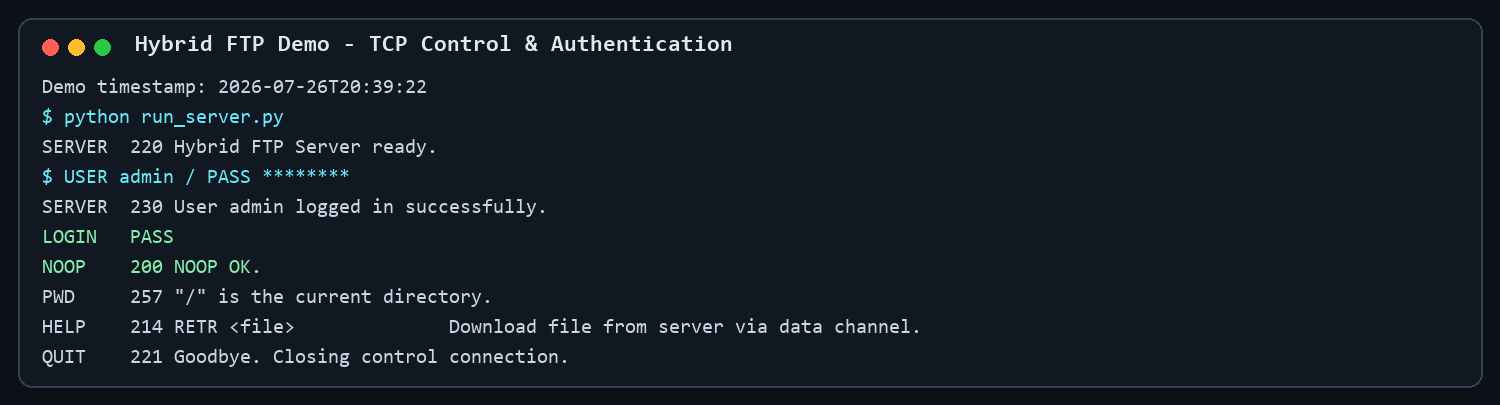
\includegraphics[width=\textwidth]{images/01-control-auth.png}
\caption{Actual control-channel authentication and session log.}
\end{figure}

\subsection{Demo B: Directory navigation}

\textbf{Objective.} Verify directory management inside the server sandbox.

\textbf{Execution.} The client executed MKD, UDP LIST, CWD, PWD, CDUP, and
RMD on \code{demo-folder}.

\textbf{Result.} Creation returned 257, the folder appeared in LIST, the
session path changed correctly, and removal returned 250. All steps passed.

\begin{figure}[H]
\centering
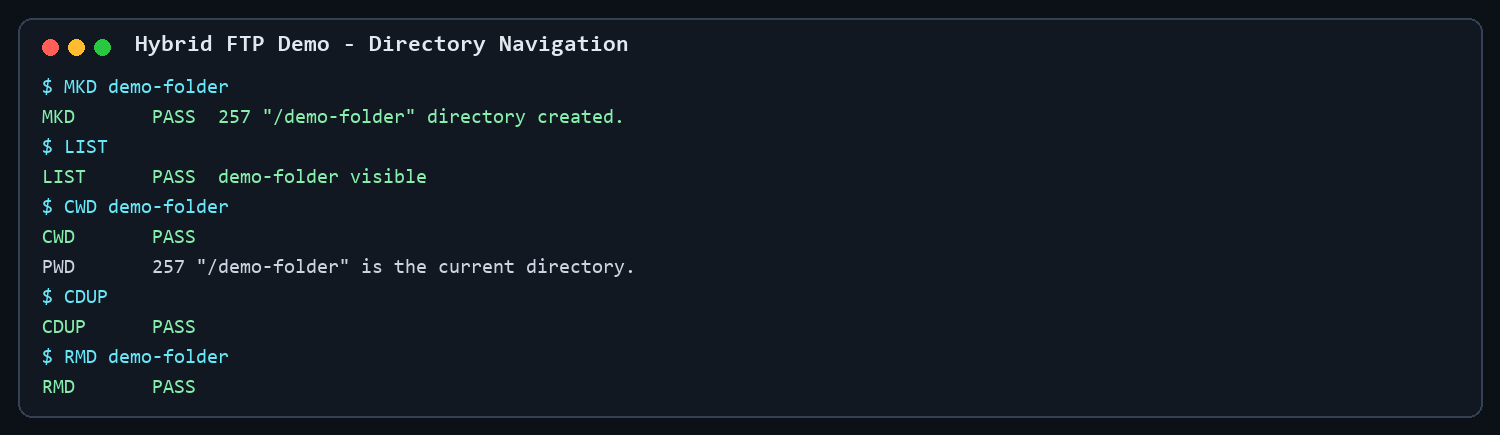
\includegraphics[width=\textwidth]{images/02-directory-navigation.png}
\caption{MKD, LIST, CWD, PWD, CDUP, and RMD evidence.}
\end{figure}

\subsection{Demo C: PASV transfer integrity}

\textbf{Objective.} Verify passive binary upload/download, metadata, and
end-to-end SHA-256.

\textbf{Execution.} Under TYPE I and PASV, the client uploaded and downloaded
a 16,384-byte file, compared its bytes, and requested SIZE, MDTM, STAT and
HASH SHA256.

\textbf{Result.} Both transfers passed, SIZE returned 16,384, metadata replies
were valid, and the local/server SHA-256 values matched.

\begin{figure}[H]
\centering
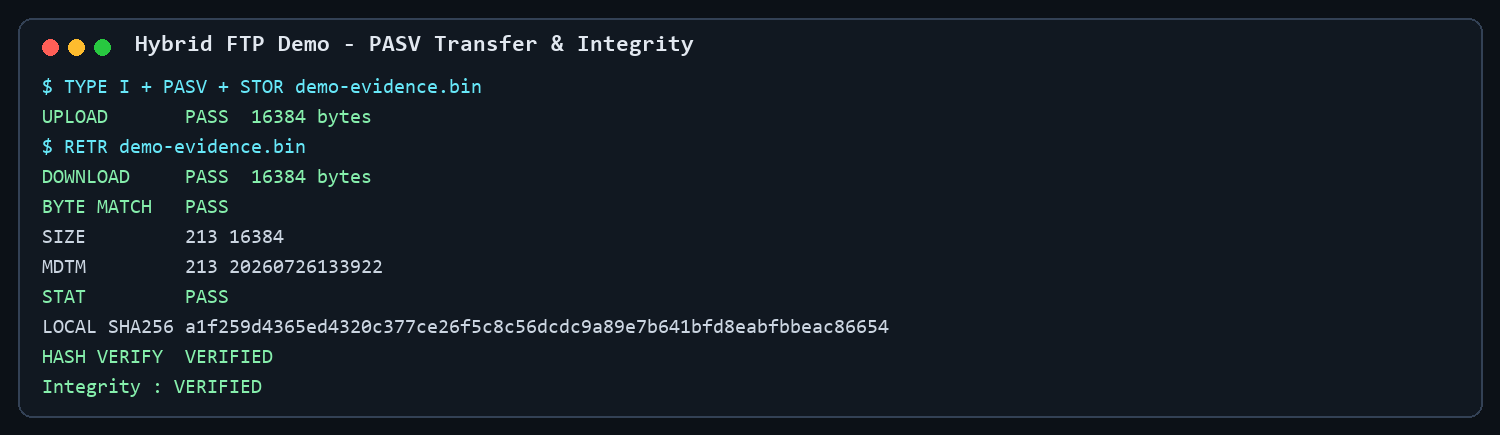
\includegraphics[width=\textwidth]{images/03-pasv-transfer-integrity.png}
\caption{PASV upload/download, metadata, and SHA-256 comparison.}
\end{figure}

\subsection{Demo D: ASCII and compressed representations}

\textbf{Objective.} Verify TYPE A canonicalisation and MODE C compression.

\textbf{Execution.} A two-line text file completed an ASCII round trip. The
binary payload then completed an upload/download under zlib compressed mode.

\textbf{Result.} ASCII upload, download, and newline comparison passed. The
decompressed binary output matched the original.

\begin{figure}[H]
\centering
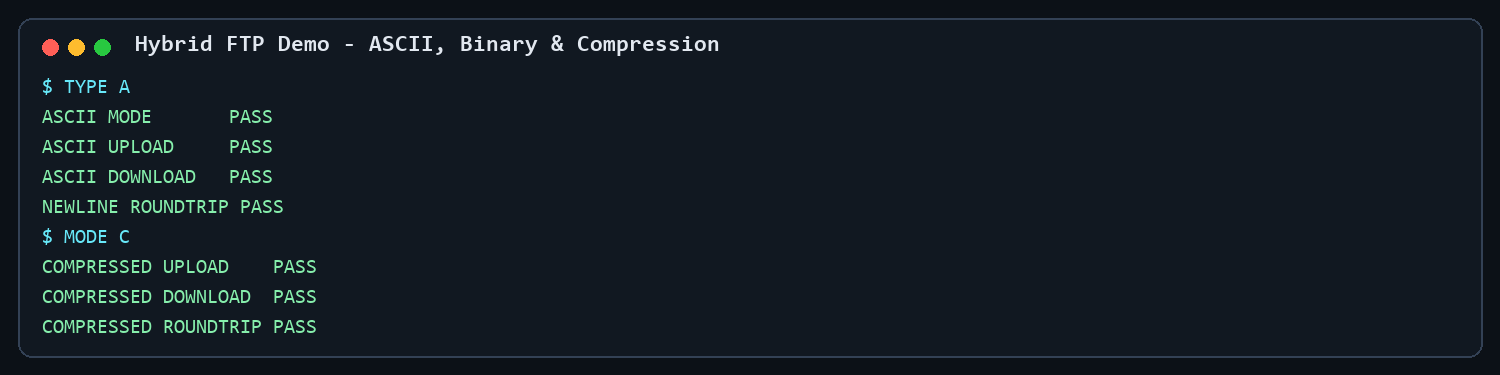
\includegraphics[width=\textwidth]{images/04-ascii-compression.png}
\caption{TYPE A newline round trip and MODE C compression.}
\end{figure}

\subsection{Demo E: Active PORT mode}

\textbf{Objective.} Verify runtime switching to the active data mechanism.

\textbf{Execution.} The client advertised its UDP endpoint with PORT. It then
uploaded, downloaded, byte-compared, and SHA-256-verified a binary file.

\textbf{Result.} PORT returned 200; both transfers and the byte comparison
passed; SHA-256 was verified.

\begin{figure}[H]
\centering
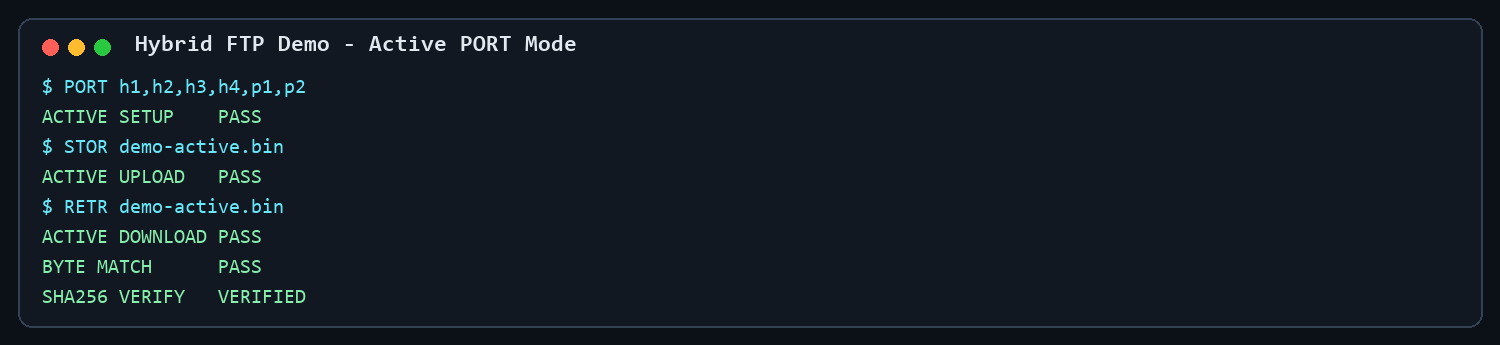
\includegraphics[width=\textwidth]{images/05-active-port.png}
\caption{Active-mode upload/download with byte and SHA-256 verification.}
\end{figure}

\subsection{Demo F: Extended file operations}

\textbf{Objective.} Verify rename, append, unique store, listing and deletion.

\textbf{Execution.} A 40-byte file was stored, renamed with RNFR/RNTO,
appended, measured, followed by STOU, NLST and deletion.

\textbf{Result.} SIZE became 80 bytes after append. The server generated a
unique filename; listing and both deletions passed.

\begin{figure}[H]
\centering
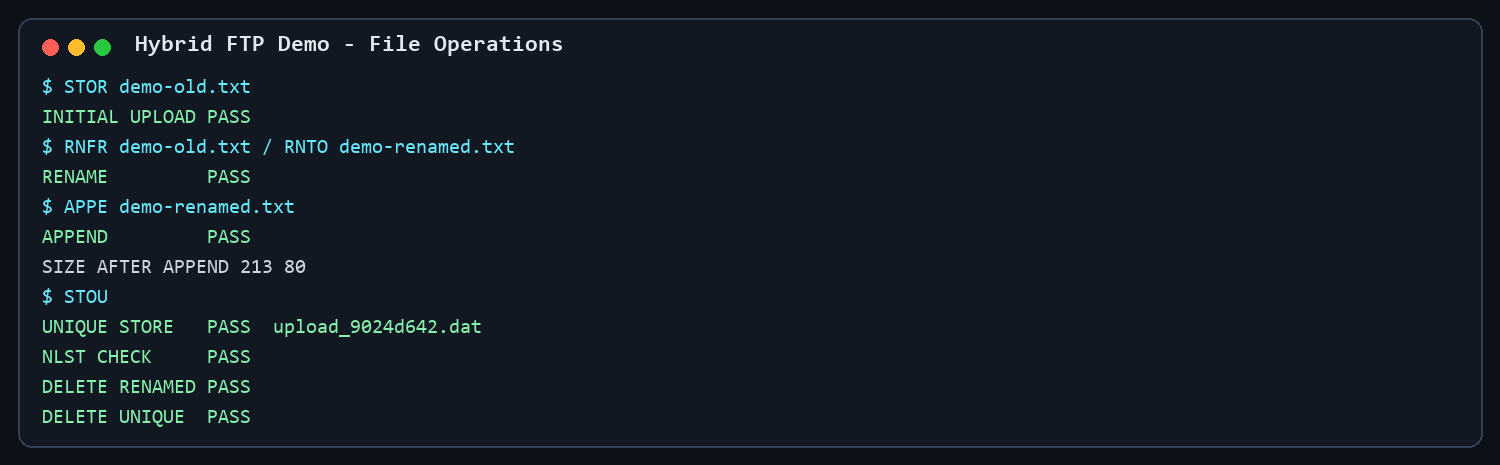
\includegraphics[width=\textwidth]{images/06-file-operations.png}
\caption{Rename, append, unique-store, listing, size, and deletion evidence.}
\end{figure}

\subsection{Demo G: Go-Back-N loss recovery}

\textbf{Objective.} Demonstrate recovery from a real missing DATA datagram.

\textbf{Execution.} A 20\% loss simulator deterministically dropped sequence
zero. The remaining sender, receiver, timer, ACK and UDP behaviour was real.

\textbf{Result.} The sender timed out at base zero, retransmitted the
outstanding flight, completed with one retransmission, and produced a
verified SHA-256 digest.

\begin{figure}[H]
\centering
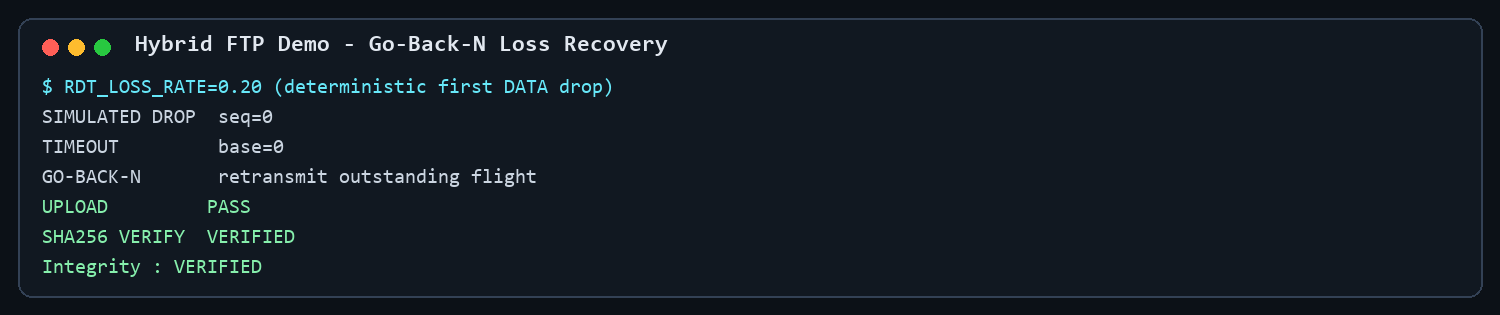
\includegraphics[width=\textwidth]{images/07-loss-recovery.png}
\caption{Deterministic DATA loss, timeout, retransmission, and verified hash.}
\end{figure}

\subsection{Demo H: Concurrent isolated sessions}

\textbf{Objective.} Verify multi-threaded session isolation.

\textbf{Execution.} Three independent clients concurrently logged in, opened
PASV endpoints, uploaded unique files, verified hashes, deleted the files,
and quit.

\textbf{Result.} All three clients passed login, upload, and SHA-256
verification. No worker timed out or produced a mismatched digest.

\begin{figure}[H]
\centering
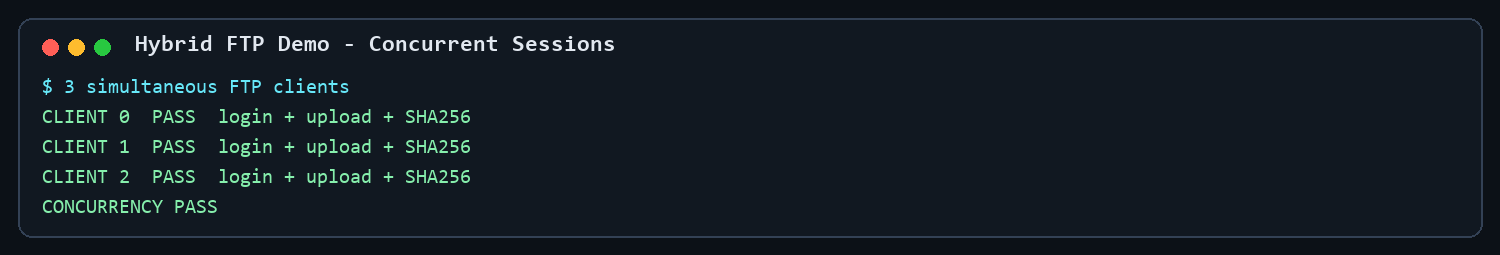
\includegraphics[width=\textwidth]{images/08-concurrency.png}
\caption{Three simultaneous authenticated client sessions.}
\end{figure}

\subsection{Evidence and test relationship}

\begin{lstlisting}
python -m unittest tests.test_core -v
python -m unittest tests.test_integration -v
python -m unittest discover -s tests -v
python tools/generate_demo_evidence.py
\end{lstlisting}

The E2E suite covers real TCP authentication, PASV/PORT UDP transfers,
binary SHA-256 verification, ASCII and compressed round trips, metadata,
STOU/APPE/rename, live ABOR, deterministic packet loss and retransmission,
three concurrent authenticated clients, and cleanup.

\begin{table}[H]
\centering
\begin{tabular}{lll}
\toprule
Demo & Requirement & Result\\
\midrule
A & TCP control and authentication & PASS\\
B & Directory management & PASS\\
C & PASV binary and SHA-256 & PASS / VERIFIED\\
D & ASCII and compression & PASS\\
E & Active PORT mode & PASS / VERIFIED\\
F & Extended file operations & PASS\\
G & Go-Back-N loss recovery & PASS / VERIFIED\\
H & Three concurrent clients & PASS\\
\bottomrule
\end{tabular}
\caption{Summary of observed demonstration results.}
\end{table}
\end{document}